\documentclass[a4paper]{article}
\usepackage{mystyle}

\addbibresource{references.bib}

\begin{document}

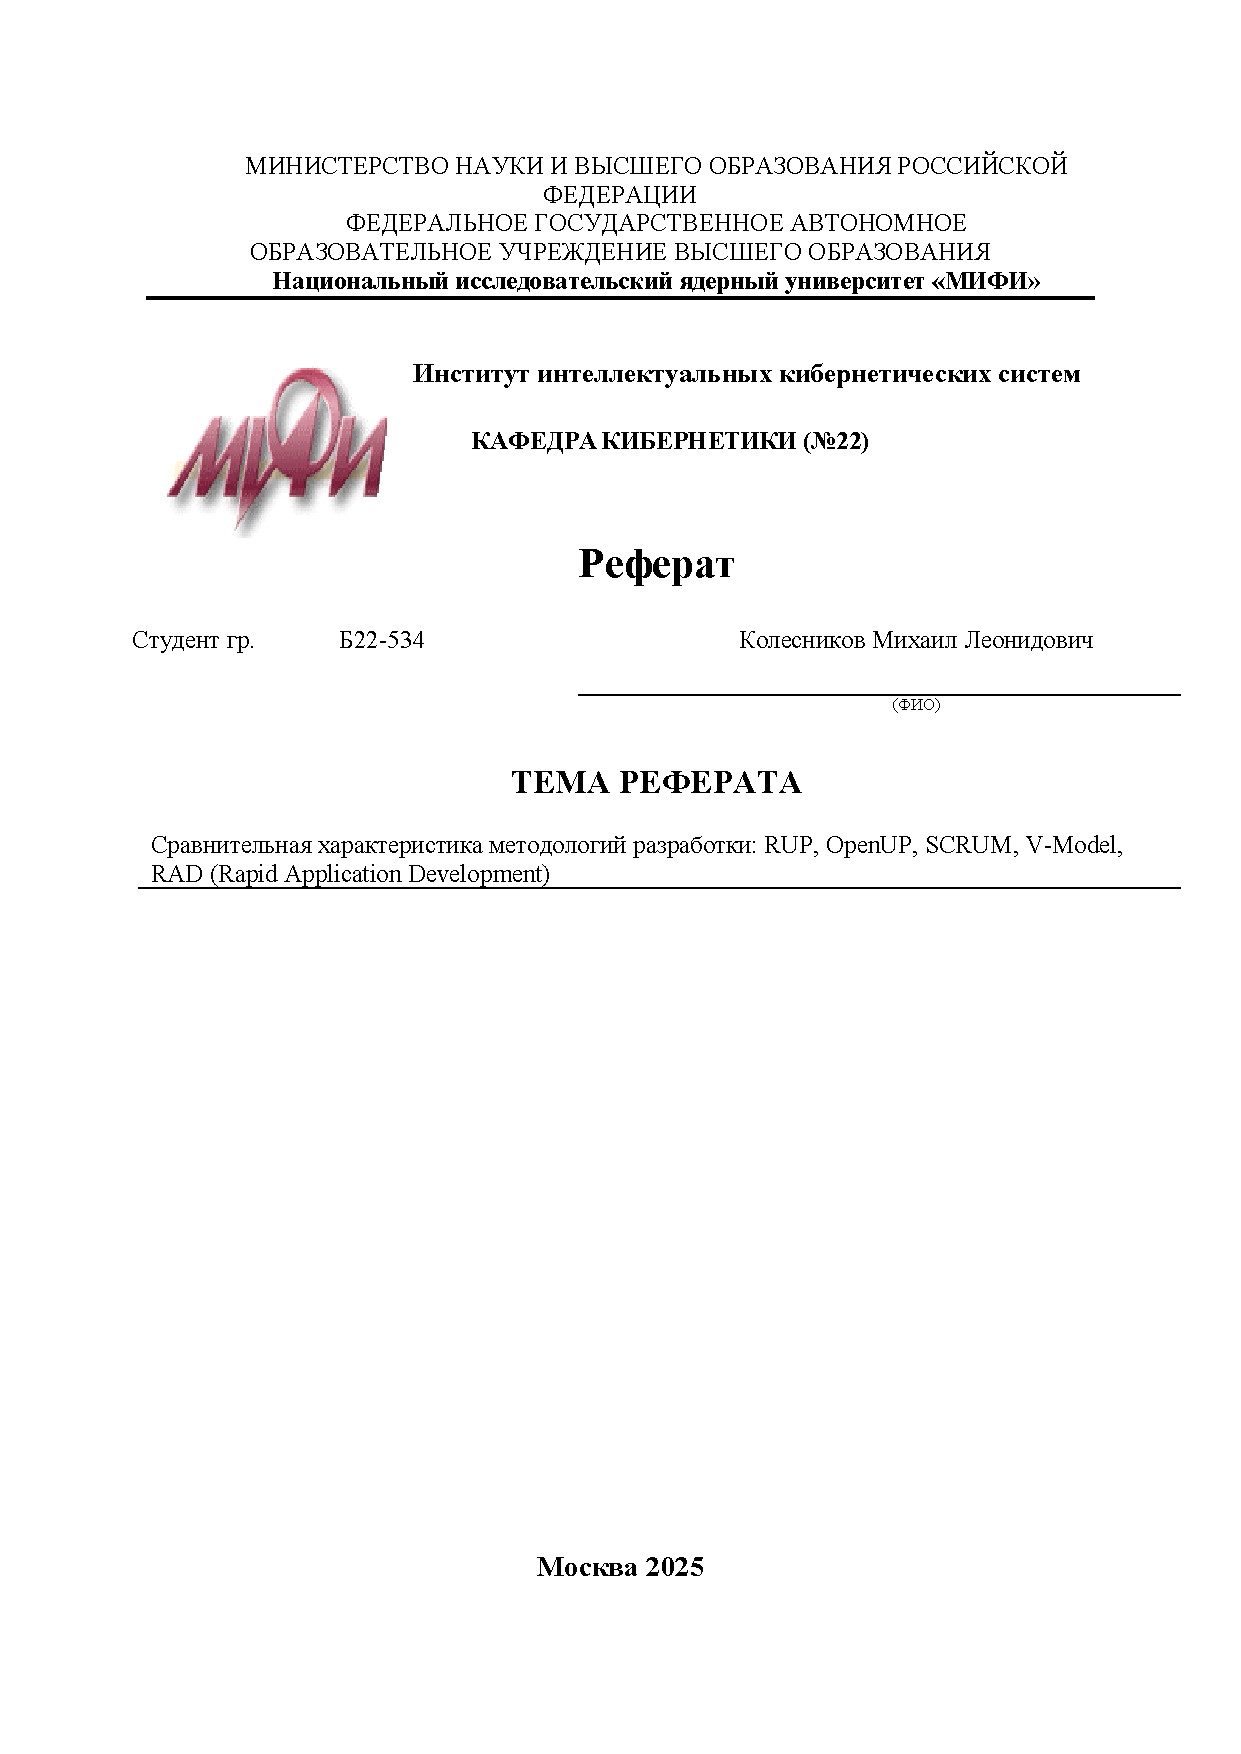
\includepdf[pages={1}]{titul.pdf}

\tableofcontents

\newpage

\section{Введение}
\input{txtFiles/1.txt}

\newpage

\section{Описание методологий разработки ПО}

\subsection{RUP (Rational Unified Process)}
\input{txtFiles/2.1.txt}

\subsection{OpenUP (Open Unified Process)}
\input{txtFiles/2.2.txt}

\subsection{SCRUM}
\input{txtFiles/2.3.txt}

\subsection{V-Model}
\input{txtFiles/2.4.txt}

\subsection{RAD (Rapid Application Development)}
\input{txtFiles/2.5.txt}

\newpage

\section{Сравнительная характеристика методологий}

\subsection{Приоритеты в каждом подходе}
\input{txtFiles/3.1.txt}

\subsection{Политики в отношении анализа и проектирования}
\input{txtFiles/3.2.txt}

\subsection{Политики в отношении написания и организации кода}
\input{txtFiles/3.3.txt}

\subsection{Политики в отношении тестирования}
\input{txtFiles/3.4.txt}

\subsection{Политики в отношении внедрения}
\input{txtFiles/3.5.txt}

\subsection{Организация взаимодействия внутри команды (или между командами)}
\input{txtFiles/3.6.txt}

\newpage

\section{Заключение}
\input{txtFiles/4.txt}

\newpage

\section*{Литература}
\printbibliography[heading=none]

\end{document}